\documentclass[main.tex]{subfiles}

\begin{document}
\pagenumbering{arabic}	% Numbering style for body

\chapter{Introduction}
\chaplabel{introduction}
\section{Background and motivation}
\seclabel{background}

It is estimated that over one hundred million landmines are currently unaccounted for in past and present conflict zones across the globe. Remaining active for many years after burial, these indiscriminate weapons are responsible for injuring thousands of civilians and military personnel each year \parencite{landmineMonitor2015}.

The Defence Science and Technology Group (DSTG) is an Australian Government organisation that applies scientific methods and technologies with the aim of defending Australia's national interests. A current focus for the DSTG is reducing the risks posed to Australian Defence Force (ADF) personnel by landmines in conflict zones. There are two primary methods of landmine detection currently employed by the ADF: manual screening with the use of a handheld metal detector, and vehicle mounted screening using Ground Penetrating Radar (GPR) arrays.
Both methods require personnel to be in close proximity to landmines due to the need for manual control of the sensors. Another major drawback to both methods is the difficulty to distinguish between landmine and non-landmine objects, which results in a large number of false positives - where a non-landmine object is incorrectly identified as being a landmine. This leads to demining operations being very time consuming as extreme care must be taken with each potential threat. The inefficiency and high risk associated with these demining operations is the major motivation for the current project. 

As a solution, the DSTG is investigating systems that can locate and identify a range of threats with increased speed and accuracy, while at the same time removing operators from potential harm. This project proposes the development of an autonomous and unmanned platform to mount landmine detection equipment, which would eliminate the risk to operators entirely. Through the use of a multi-sensor system consisting of a metal detector and a GPR, combined with sensor fusion, the aim will be to reduce false positives thereby increasing detection accuracy.

\nomenclature{DSTG}{Defence Science and Technology Group}% 
\nomenclature{ADF}{Australian Defence Force}% 
\nomenclature{GPR}{Ground Penetrating Radar}%

\section{Project goal}
\seclabel{projectGoal}

The goal of this project is to develop an autonomous platform for landmine detection, with a focus on the reduction of false positives. The project objectives necessary to achieve this goal are described below.
 
\subsection{Primary objectives}
\seclabel{primary}
An autonomous platform must be produced to meet the project goal. This platform should be capable of traversing the complex terrain expected in landmine-afflicted areas. To be fully autonomous, the platform must also be capable of being operated remotely, or by computer software under the supervision of an operator. The detection system must be capable of providing some feedback mechanism to allow the operator to sufficiently assess the situation to provide adequate supervision.

The computer software developed to autonomously guide the remote platform must be capable of safely navigating an active minefield, and so needs to be able to respond to instructions quickly in order to avoid accidentally detonating a landmine. The software must behave predictably while autonomously controlling the platform in order to allow an operator to easily supervise the device. The software must also be capable of navigating the platform to arbitrary geographic locations by performing suitable manoeuvres or following instructions from an operator.

The remote platform must also be capable of being equipped with any necessary sensory equipment to detect landmines, with respect to payload weight and size. 
The mounting of this equipment must also be capable of allowing the sensory equipment to operate effectively, isolated from noise, vibrations, and any other interfering signals. 
The output from these sensors would then be used in conjunction with a software algorithm trained to identify landmines and to provide a better object classifying multi-sensor system relative to naive individual sensors.

This project vision was used to produce a set of objectives for a delivered system which successfully fulfils the project goal, and to determine acceptance criteria of the project deliverables. 
These objectives are formally defined as:

\begin{enumerate}
\item \textbf{Selection and subsequent modification of an existing platform for control via a remote device}\\ 
Modifications will be made to a commercially available vehicle to allow for remote, electronic control of all subsystems associated with vehicle motion.
An existing platform will be modified rather than constructing a vehicle to restrict project scope and accommodate time constraints. 
This requirement will be deemed completed once all mechanical or electrical systems on the platform necessary for autonomous navigation can be reliably controlled by a remote electronic system, and with sufficient level of control to permit further development of autonomous systems. 
Selection of the device is expected to be completed within one month of confirmation of the project budget, and modifications are expected to be complete within two months of platform selection.

\item \textbf{Software development for platform automation and basic navigation, allowing for the platform to travel autonomously under supervision from an operator}\\ 
A software system will be developed that will be able to utilise the actuators and other electronic controls installed on the remote platform in order to produce autonomous vehicle motion. 
Due to safety concerns, a software simulator will be required to allow preliminary testing of this software in a low-risk environment. 
This requirement will be deemed complete upon the adequate completion of both a virtual platform simulator and an autonomous navigation system. 
Adequate completion of the virtual platform will be determined by confirmation that the simulator accurately represents the expected motion of the physical platform under the same inputs.
The autonomous software will be expected to control the virtual platform’s motion such that it follows a path pre-defined by a series of points, without deviating from the path in a way that would cause the platform to cover ground that is not previously covered by the landmine detection sensors. 
It is expected that this software system, as well as the virtual platform for simulation of autonomous behaviour, will be able to be completed within six months from the selection of the remote platform.

\item \textbf{Automatic traversal of a user defined path or region}\\ 
The operator of the landmine detection system should be able to define an arbitrary path or enclosed geographical region. 
The autonomous software will be extended to allow for path definitions to be changed during run-time. 
An additional software system will be created with the ability to select a region, defined as a series of points, which results in complete scanning coverage of the region.
Acceptance criteria for this objective are that a system is provided which allows an operator to define paths or scanning zones, that the route planning software can produce a path which systematically covers arbitrary zones resulting in 100\% sensor coverage, and that the autonomous navigator will be capable of following this path as confirmed using the virtual platform.
Development of this system is expected to be completed concurrently with the development of the autonomous software, and able to be completed within one month of the completion of the navigation software.

\item \textbf{Modification of an existing platform to accommodate landmine detection sensors}\\ 
The landmine detection sensors are required to be attached to the platform in such a way that they can be used to scan ground not previously traversed by the vehicle, and that the movement of the vehicle does not interfere with the sensing abilities of the detectors. 
The acceptance criteria for this requirement are that the sensors are suitably attached to the platform such that they cannot detach or displace during operation, and that the change in background signal noise resulting from attachment to the remote platform or proximity to other sensors is not discernible from typical levels. 
This requirement is expected to be completable within one month of receipt of the vehicle and of the detection sensors.

\item \textbf{Software development for detection and identification of subsurface objects, with a focus on reducing the number of false positives}\\ 
A software system will be developed which will be capable of processing real-time data from the detection sensors, with an ability to identify anomalous signals corresponding to non-landmine objects. 
The software will be required to use a metrics based system to attempt to classify detections as either landmine or non-landmine. 
Acceptance criteria will be tested by live trials on test objects. 
This requirement will be deemed complete once the detection software is capable of detecting subsurface objects using real-time data. 
The classification software will be required to achieve 100\% correct classification of detected landmines while also reducing the false-positive identification rate, demonstrating an improvement over naive object-detection-only systems. 
The detection software must be able to achieve improved detection when using multiple sensors, or the classification software must be able to achieved reduced false classification, demonstrating the value of the multi-sensor system. 
This requirement represents a highly experimental aspect of the project, and as such completion expectations will depend on the results of preliminary testing. 
\end{enumerate}

\subsection{Extended objectives}
\seclabel{extendedObjectives}
Where time and other resources permit, these requirements will be extended with optional objectives that would progress the project beyond a proof-of-concept system, creating a deliverable that would more closely represent a completed, commercial system. 
These extended requirements are below:

\begin{enumerate}
\item \textbf{Development of a tablet application that allows for communication and control of the platform and sensor systems}\\ 
Rather than receiving information on a computer, a portable handheld device such as a tablet would be used. 
A dedicated application will be developed, allowing for even an unskilled operator to carry out a complex mission. 
The operator will be able to control and monitor the progress of the platform in real time, and once an object is detected by the sensor system, the operator will also be notified. 
A GPS coordinate will be assigned to the object, and based on the returned sensor data, the operator can make an informed decision about how to proceed.

\item \textbf{Provision of a live video feed to the operator}\\ 
A live video feed allows for an operator to have a better understanding of the operating environment. 
A camera will be installed on the platform, and the output will be integrated with the developed tablet application. 
This will allow the operator to detect and respond appropriately to unknown obstacles in the search area. 

\item \textbf{Physical marking of landmine locations by the platform at the time of detection}\\ GPS coordinates alone may not provide sufficient precision for identifying the location of landmines. 
An electro-mechanically powered system that physically marks the location would allow demining personnel to identify this location more clearly.

\end{enumerate}

\section{Scenario of operation}
\seclabel{SoO}
This section will look at real world environments that the platform could be expected to operate in. In addition, the mission profile, which is the intended use case for the platform, is presented. Based on these, a set of performance specifications are developed.  

\subsection{Operating environments}
\seclabel{operatingEnvironments}
There are a large number of countries in which ADF personnel are deployed, all of which have differing terrain, vegetation, soil types, landmine types and sizes of landmine affected areas. Since it is impossible to develop a platform that suits all real world operating conditions, the Middle Eastern region is selected to be investigated further, since this is the location to which the largest number of ADF personnel are deployed \parencite{AustralianGovernment2016}. 

The Middle East is heavily affected by landmines and unexploded ordnance due to many years of conflict (Smith 2016). There are an estimated 23 million landmines buried throughout this region, with landmine technologies ranging back to World War II \parencite{Khamis13}. As a result, landmines range from plastic and composite anti-personnel mines to high metal content anti-tank mines. The primary goal of burying landmines is to conceal their location, therefore they are typically buried from 5 cm to 15 cm below the surface, depending on the time available to bury them and the terrain properties.

Most landmine affected areas within the Middle East are predominantly flat, sandy and gravely expanses \parencite{Nahrawy2011}. They are covered with loose or compacted small granular soils that have little to no nutritional value for vegetation, leaving the areas sparsely covered by plants (Khan 2010).  
Egypt and Iran are two such environments that are considered, both of which are heavily affected by landmines.

\subsubsection{Eqypt}
\seclabel{Egypt}

Egypt is listed as the country most contaminated by landmines, with an area of roughly 25,000 square kilometres containing both anti-tank and anti-personnel mines \parencite{Rushfan2008}. The majority of these landmines were placed during World War II and consist of high metal content anti-tank and anti-personnel mines \parencite{Khamis13}. %The main contaminated areas are along the North coast and the Sinai Peninsula. These areas represent 22\% of the total area of Egypt and consist predominantly of lithosols with large flat expanses of sandy land \parencite{Nahrawy2011}. Temperatures in excess of 50 degrees are common, making it difficult for demining personnel to operate for extended periods of time \parencite{Khamis13}. 
%Over time, shifting sands allow these landmines to sink deeper to depths of up to 2 metres, beyond the range of most landmine detection techniques \parencite{Khamis13}. 
%The chosen platform would then be required to travel over sandy terrains and over small obstacles such as rocks, with the sensors being able to detect landmines through sandy and loose soil to depth of up to 15 cm. 

\subsubsection{Iran}
\seclabel{Iran}
Iran has an area of approximately 18,000 square kilometres of land contaminated with 12-16 million landmines left over from the 1980-1988 Iran-Iraq conflict, consisting of composite and non-composite landmines \parencite{landmineMonitor2015}. %The main areas of contamination are western provinces such as Khuzestan, which has mountainous terrain and sandy soils \parencite{Aman16}. 
%Both anti-tank and anti-personnel mines can be found, with shifting sands causing landmines to sink to depths greater than 80 cm \parencite{Aman16}.

%\textcolor{red}{This paragraph and the one before it need more information about terrain, vegetation, soil type, moisture, mine type, \textbf{mine depths}, obstacles, gradient, whatever else can be found! These should then lead provide the basis for the details presented at the start of the mission profile. Or maybe have an additional subsection, which describes the chosen operating environment... - RK} 


\subsection{Mission profile}
\seclabel{MissionProfile}
A typical demining operation requires personnel to clear a path or area, ensuring it is safe for ground troops and vehicles to pass over. The mission profile developed for the platform, shown in \Figref{mission}, is based off of typical conditions in the Middle East, and will form the basis of many of the project's design requirements.
\begin{quote}The mission takes place in a region with dry, sandy soils and level terrain unobstructed by vegetation or obstacles, such as a road or open field. A number of types of landmines, including high and low metal content anti-personnel and anti-tank mines, can be found buried at depths of up to 15 cm. The operator will use a remote device to select waypoints that define a path or the boundaries of an area of interest. The platform will travel out to this path or area, then autonomously navigate it. Using the onboard sensor suite, the platform scans the area at an operational speed of 5 km/h. Whenever a detection is made, the platform comes to a stop in a safe distance and logs the GPS coordinates of the location, with a positional error of less than 0.5 m. Sensor data and a confidence interval are sent to the operator in real time, giving the likelihood of the detected object being a landmine. Once the operator instructs the platform to resume, it continues to scan the area. Over time, a map of the scanned region showing all detected objects is developed using the sensor data. At any point the operator can abort the mission, or take manual control of the platform.
\end{quote}

\begin{figure}[ht]
\centering
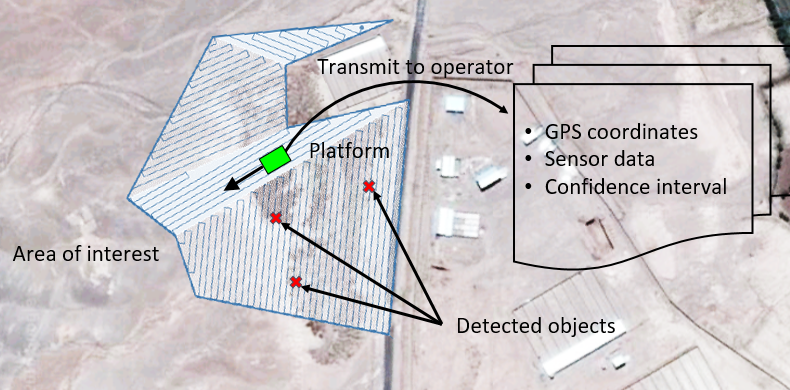
\includegraphics[width=\textwidth]{1-Introduction/SoO.PNG}
\caption{Schematic of mission profile}
\figlabel{mission}
\end{figure}

\subsection{Performance specifications}
\seclabel{performance}
Knowing the basic operating environment and mission profile, performance specifications can be defined, encompassing the platform and sensor systems. The operating environments were utilised to determine the types of terrains, landmines and depth requirements for the project, while the mission profile was used to determine the platform requirements and necessary communication devices.   

\subsubsection{Platform}
\seclabel{platform}
In order to be able to autonomously navigate a region of interest and meet the project objectives, the platform must meet the following requirements: 
\begin{itemize}
 \item Carry a total payload of 100 kg. A pair of metal detector and GPR arrays with their respective control boxes have an estimated gross weight of 80 kg. This allows 20 kg for any mounting structures, electronics and computers.
 \item Travel off-road in regions with dry sandy soils and level unobstructed terrain with little to no vegetation, as described in the operating environment.
\item Travel in a straight line, both forwards and reverse, and perform turns while maintaining an operational speed of 5 km/h, as required in the mission profile. 
\item Be manoeuvrable enough to navigate the region of interest, yet controllable enough that in case of an emergency, it can come to a complete stop from its operational speed with no risk of detonating a landmine.
\end{itemize}

\subsubsection{Sensors}
\seclabel{sensors} 
The requirements for the sensor system are also derived from the operating environment and mission profile:
\begin{itemize}
\item Detect high and low metal content anti-personnel and anti-tank mines, as are commonly found in the Middle East. 
\item Identify landmines at depths of up to 15 cm at an operational speed of 5 km/h, as specified in the mission profile.
\item Discriminate between different landmines and other objects, aiming to minimise the number of false positives detected as described by the project goal.
\end{itemize}

\section{Project scope}
\seclabel{projectScope}

%Acceptance criteria: The conditions that must be met before project deliverables are accepted.
%Deliverables: The products, services, and/or results your project will produce (also referred to as objectives).
%Project Exclusions: Statements about what the project will not accomplish or produce.
%Constraints: Restrictions that limit what you can achieve, how and when you can achieve it, and how much achieving it can cost.
%Assumptions: Statements about how you will address uncertain information as you conceive, plan, and perform your project.

The aim of this project is to demonstrate the feasibility of a concept that incorporates an autonomous platform and a real time multisensor landmine detection system. It is not intended for the final design solution to be a commercially viable device that is ready to be deployed for the ADF. 

The successful delivery of the completed platform and accompanying software will require design, construction and testing. Testing of the sensor system will be limited to horizontally placed landmines and readily available soil types. Higher level automation processes such as object avoidance will not be considered. 
\end{document}